%!TEX root = bambi-thesis.tex
The PX4 firmware offer a great Software-In-The-Loop  simulation environment which was fundamental for the software development. It guarantee a real-time, safe and convenient way to test the software implementation without all the risks related to a real flight.\\

\section{Simulation Environment} % (fold)
\label{sec:simulation_environment}
The simulation environment consist of:
\begin{itemize}
 	\item PX4 SITL: The PX4 simulated hardware which reacts to the simulated given input exactly as it would react in the reality and issues the output as a percentage of the total thrust that every rotor has to provide.
 	\item Gazebo: The dynamics simulator that is used by the SITL. This software reads the PX4 output and, by elaborating the modeled dynamics, provides the simulated input to the PX4. This allows for a quite accurate simulation of the real model behavior during flight.
 \end{itemize}
 The different parts of the system (\autoref{fig:SITL-architecture}) are connected via UDP, and can be run on either the same computer or another computer on the same network. The communication protocol is MAVLink (see appendix \ref{appendix:mavlink}).
 \begin{figure}[ht]
    \centering
    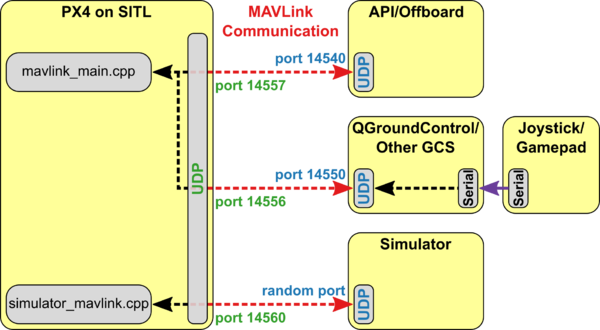
\includegraphics[width=.7\textwidth]{figures/C4/Px4_sitl_overview}
    \caption{SITL with Gazebo architectural scheme}
    \label{fig:SITL-architecture}
\end{figure}
% section simulation_Environment (end)

